\documentclass[]{article}
\usepackage{graphicx}
\usepackage[margin = 1.5 cm]{geometry}
\usepackage{color}
\newcommand{\BlueText}[1]{\textcolor{blue}{#1}}


\begin{document}
\noindent \BlueText{\textbf{Exercise 3:} Attempt to replicate the following in black text.
(\textbf{\underline{HINT:}} You are going to need the \texttt{graphicx} package. Also note that the margins for this document are 1.5 cm all the way around which can be done using the \texttt{geometry} package.}
\vspace{1cm}

\noindent Below is my scientific idol. \BlueText{$\leftarrow$ download your own photo to include but make sure it is in the same folder as your .tex document}

%%%%%%%%%%%%%%%%
%%%% DONE: Add a figure 
\begin{figure}[h]
\centering
	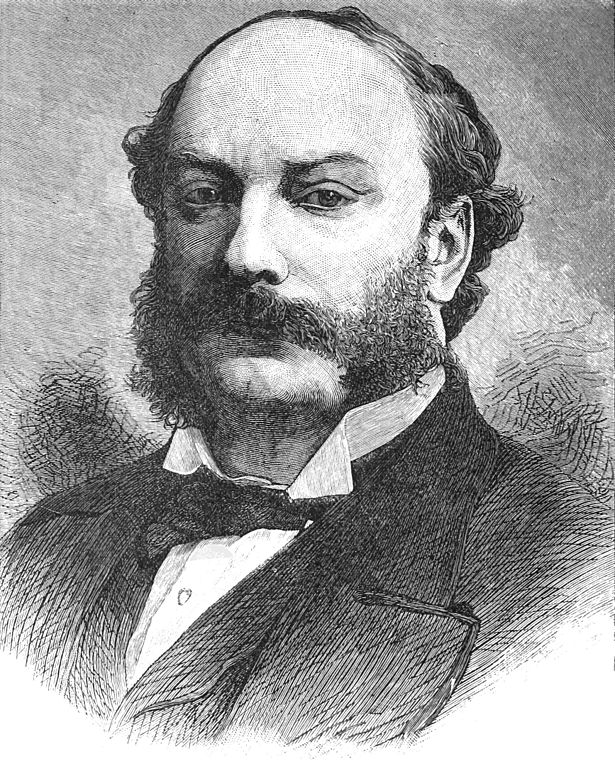
\includegraphics[width = 0.5\textwidth] {./Rayleigh.jpg}
	\caption{\textit{The} Lord Rayleight}
\end{figure}

\noindent Below is a list of three random US presidents and some information regarding them.

\begin{table}[h]
\centering
\begin{tabular}{| c | c | c | c | c |}
	\hline
	\textbf{No.} & \textbf{Name} & \textbf{Party} & \textbf{Term Start} & \textbf{Term End} \\ \hline
	2 & John Adams & Federalist & March 4, 1797 & March 4, 1801 \\ \hline
%%%%%%%%%%%%%%%%
%%%% DONE: Add enteries to a table
	25 & William McKinley & Republican & March 4, 1897 & September 14, 1901 \\ \hline
	39 & Jimmy Carter & Democratic & January 20, 1997 & January 20, 1981 \\ \hline
\end{tabular}
\end{table}

\end{document}